\def\eeprepfigure{1}
\def\eepH{400}
% eeprep.com CircuiTikZ house style — "Clean modern textbook"   (UNTESTED here: no TeX on build box)
% Build: lualatex fig.tex  &&  dvisvgm --pdf --font-format=woff2 --exact-bbox -o fig.svg fig.pdf
%   (or: pdftocairo -svg fig.pdf fig.svg  — outlines text; use if fonts must be embedded)
% Requires: TeX Live 2023+, circuitikz ≥ 1.6, fontspec, unicode-math, Newsreader + Inter + JetBrains Mono installed.
\documentclass[border=4pt]{standalone}
\usepackage{fontspec}
\usepackage{unicode-math}
\setmainfont{Newsreader}[ItalicFont={Newsreader Italic}]
\setsansfont{Inter}
\setmonofont{JetBrains Mono}
\setmathfont{STIX Two Math}                       % complete math coverage
\setmathfont{Newsreader Italic}[range=it/{latin,Latin}]  % variables match site serif italic
\setmathfont{Newsreader}[range=up/{latin,Latin,num}]
\usepackage{xcolor}
% Sentinel colours — the site <Diagram> component maps these hex values to CSS vars (theme-spec §7.6)
\definecolor{eepink}{HTML}{16233A}
\definecolor{eepaccent}{HTML}{A3201D}
\definecolor{eepmute}{HTML}{838C9A}
\definecolor{eepfill}{HTML}{FFFFFF}
\usepackage[american,siunitx,RPvoltages]{circuitikz}
\usepackage{siunitx}
\sisetup{detect-all, text-family-to-math=false}
\ctikzset{
  bipoles/thickness=1,            % same as wires
  bipoles/length=1.1cm,
  resistors/scale=0.8, capacitors/scale=0.75, sources/scale=0.85,
  csources/scale=0.85, grounds/scale=0.9,
  nodes width=0.06,               % node dot size
  voltage/american label distance=0.6,
  label/align=straight,
  color=eepink,
}
\tikzset{
  every picture/.style={line width=1.31pt, line cap=round, line join=round, color=eepink, font=\normalsize},
  % 1.31pt ≈ 1.75px at 1:1. Draw at final size: one-loop schematic ≈ 10.5cm wide (≈ 400pt ≈ 560px)
  val/.style={font=\ttfamily\footnotesize, text=eepaccent},   % "1 kΩ"
  pm/.style={font=\sffamily, text=eepmute},                    % + / −
  hl/.style={color=eepaccent},                                  % ONE highlighted element per figure
  ann/.style={font=\sffamily\footnotesize, text=eepmute},
}
\newcommand{\val}[1]{\textcolor{eepaccent}{\ttfamily\footnotesize #1}}

% Resume figures define \eeprepfigure and \input this file for the house
% colours, fonts, and line weight, then draw their own picture.
\ifdefined\eeprepfigure
  \expandafter\endinput
\fi

% ---- example (delete when reusing) ----
\begin{document}
\begin{circuitikz}
  \draw (0,0) to[sV, l_=$v_{\mathrm{in}}$, invert] (0,3)
        to[short, i>^=$i$] (1.5,3)
        to[R, l=$R$, a=\val{1 k$\Omega$}] (4,3) -- (5.5,3)
        to[short, -o] (7,3);
  \draw (5.5,3) node[circ]{} to[C, l_=$C$, a^=\val{100 nF}] (5.5,0) node[circ]{};
  \draw (0,0) -- (7,0) node[ocirc]{};
  \draw (2.2,0) node[circ]{} node[ground]{};
  \draw (7,3) to[open, v^=$v_{\mathrm{out}}$] (7,0);
\end{circuitikz}
\end{document}

% Colours and text helpers for the resume figures.
% Input after src/diagrams/style/circuitikz-preamble.tex.
% Define \eepdark before this file for the dark sentinels.
% Ink, accent, fill, and the 1.31pt line weight come from the house preamble.
% Light secondary text uses the approved mockup gray. Dark uses the theme mute.
% The static Newsreader cut names its bold face, which fontspec does not infer.
\setmainfont{Newsreader}[
  BoldFont={Newsreader Bold},
  ItalicFont={Newsreader Italic},
  BoldItalicFont={Newsreader Bold Italic},
]
\ifdefined\eepdark
  \definecolor{eepink}{HTML}{ECEEF2}
  \definecolor{eepaccent}{HTML}{E06A5F}
  \definecolor{eepmute}{HTML}{8F95A0}
  \definecolor{eepfill}{HTML}{131C2E}
  \definecolor{eeprule}{HTML}{3B4352}
  \definecolor{eepsoft}{HTML}{1C2537}
  \definecolor{eepdont}{HTML}{8F95A0}
\else
  \definecolor{eepmute}{HTML}{5E636C}
  \definecolor{eeprule}{HTML}{D3D7DE}
  \definecolor{eepsoft}{HTML}{ECEEF2}
  \definecolor{eepdont}{HTML}{838C9A}
\fi

% The picture uses a normal y-up axis. Pass y as in the mockup (y down).
% Each figure sets \eepH to a value past the lowest mockup y.
% #1 x  #2 baseline y (down)  #3 colour  #4 font commands  #5 text
\newcommand{\up}[5]{%
  \node[anchor=base west, inner sep=0pt, outer sep=0pt, text=#3] at (#1,{\eepH-(#2)}) {#4#5};%
}
% Drawn marks. Inter has no check or ballot x, and the house serif does not either.
\newcommand{\tick}[1]{\tikz[baseline=-0.12ex]{\draw[#1,line width=1.35pt,line cap=round,line join=round] (0,0.16em)--(0.18em,0)--(0.52em,0.5em);}\hspace{0.4em}}
\newcommand{\cross}[1]{\tikz[baseline=-0.15ex]{\draw[#1,line width=1.15pt,line cap=round] (0,0)--(0.42em,0.42em) (0,0.42em)--(0.42em,0);}\hspace{0.4em}}
% A y-down rectangle: #1 x1 #2 y-top #3 x2 #4 y-bottom
\newcommand{\boxdn}[4]{%
  \draw (#1,{\eepH-(#4)}) rectangle (#3,{\eepH-(#2)});%
}

\usetikzlibrary{arrows.meta}
\begin{document}
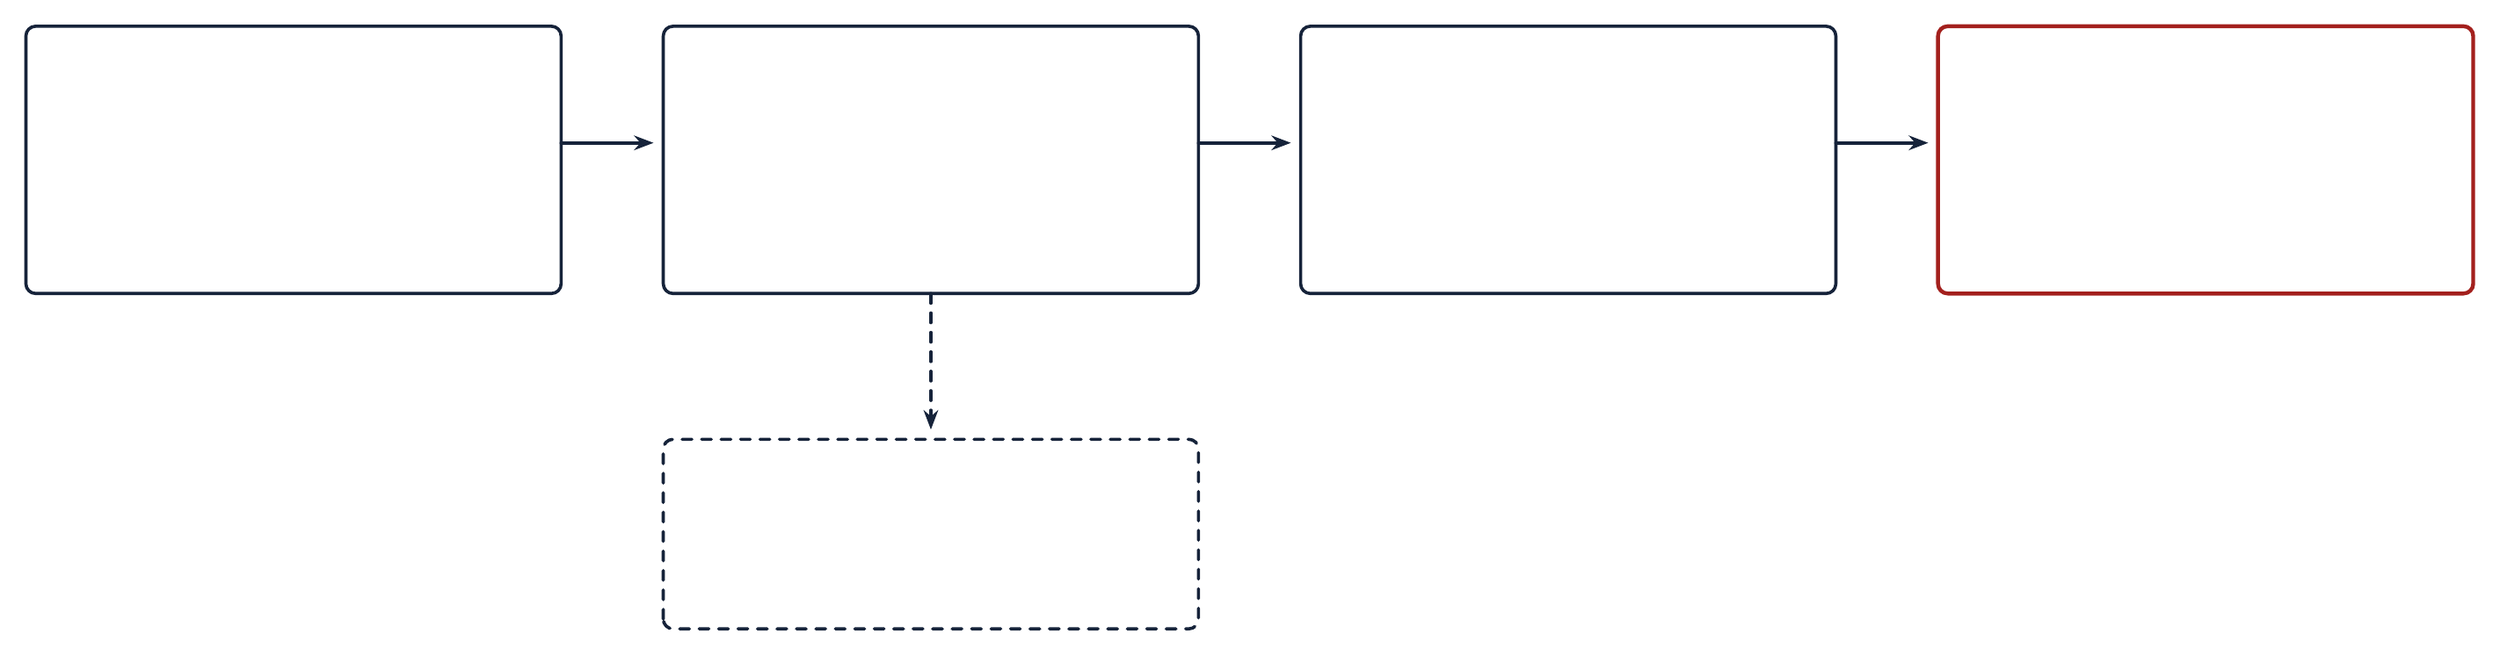
\begin{tikzpicture}[x=1pt,y=1pt,line cap=round,line join=round]
  \up{0}{16}{eepaccent}{\sffamily\bfseries\fontsize{12}{14}\selectfont\addfontfeature{LetterSpace=12}}{FIGURE 1 · HOW A RESUME GETS READ}
  \up{0}{52}{eepink}{\rmfamily\bfseries\fontsize{26}{31}\selectfont}{Software stores it. People read it.}

  % Cards follow the approved mockup, shifted down 78pt for the title.
  \draw[rounded corners=4pt, fill=eepfill] (1,{\eepH-248}) rectangle (221,{\eepH-138});
  \draw[rounded corners=4pt, fill=eepfill] (263,{\eepH-248}) rectangle (483,{\eepH-138});
  \draw[rounded corners=4pt, fill=eepfill] (525,{\eepH-248}) rectangle (745,{\eepH-138});
  \draw[rounded corners=4pt, draw=eepaccent, line width=1.6pt, fill=eepfill] (787,{\eepH-248}) rectangle (1007,{\eepH-138});

  \draw[-{Stealth[length=8pt,width=6pt]}] (221,{\eepH-186}) -- (259,{\eepH-186});
  \draw[-{Stealth[length=8pt,width=6pt]}] (483,{\eepH-186}) -- (521,{\eepH-186});
  \draw[-{Stealth[length=8pt,width=6pt]}] (745,{\eepH-186}) -- (783,{\eepH-186});

  \draw[dashed, dash pattern=on 4pt off 4pt, -{Stealth[length=8pt,width=6pt]}] (373,{\eepH-248}) -- (373,{\eepH-304});
  \draw[rounded corners=4pt, dashed, dash pattern=on 4pt off 4pt] (263,{\eepH-386}) rectangle (483,{\eepH-308});

  \up{15}{118}{eepmute}{\sffamily\fontsize{11}{13}\selectfont\addfontfeature{LetterSpace=13.6}}{STEP 1}
  \up{277}{118}{eepmute}{\sffamily\fontsize{11}{13}\selectfont\addfontfeature{LetterSpace=13.6}}{STEP 2}
  \up{539}{118}{eepmute}{\sffamily\fontsize{11}{13}\selectfont\addfontfeature{LetterSpace=13.6}}{STEP 3}
  \up{801}{118}{eepaccent}{\sffamily\fontsize{11}{13}\selectfont\addfontfeature{LetterSpace=13.6}}{STEP 4}

  \up{17}{172}{eepink}{\sffamily\bfseries\fontsize{16}{19}\selectfont}{You apply}
  \up{17}{196}{eepmute}{\sffamily\fontsize{13.5}{16}\selectfont}{Apply early. One manager}
  \up{17}{214}{eepmute}{\sffamily\fontsize{13.5}{16}\selectfont}{reads about the first 150.}

  \up{279}{172}{eepink}{\sffamily\bfseries\fontsize{16}{19}\selectfont}{The ATS stores it}
  \up{279}{196}{eepmute}{\sffamily\fontsize{13.5}{16}\selectfont}{At many companies, it stores}
  \up{279}{214}{eepmute}{\sffamily\fontsize{13.5}{16}\selectfont}{your resume rather than}
  \up{279}{232}{eepmute}{\sffamily\fontsize{13.5}{16}\selectfont}{auto-rejecting it.}

  \up{541}{172}{eepink}{\sffamily\bfseries\fontsize{16}{19}\selectfont}{A recruiter skims it}
  \up{541}{196}{eepmute}{\sffamily\fontsize{13.5}{16}\selectfont}{Companies, titles, and dates}
  \up{541}{214}{eepmute}{\sffamily\fontsize{13.5}{16}\selectfont}{get read first.}

  \up{803}{172}{eepink}{\sffamily\bfseries\fontsize{16}{19}\selectfont}{A manager reads it}
  \up{803}{196}{eepmute}{\sffamily\fontsize{13.5}{16}\selectfont}{Fast, often against hundreds}
  \up{803}{214}{eepmute}{\sffamily\fontsize{13.5}{16}\selectfont}{of other resumes.}

  \up{279}{336}{eepink}{\sffamily\bfseries\fontsize{14}{17}\selectfont}{Knockout questions}
  \up{279}{358}{eepmute}{\sffamily\fontsize{13}{16}\selectfont}{Form answers, like a clearance,}
  \up{279}{374}{eepmute}{\sffamily\fontsize{13}{16}\selectfont}{can cut you automatically.}
  \up{385}{282}{eepmute}{\sffamily\fontsize{12}{14}\selectfont}{automatic cuts happen here}
\end{tikzpicture}
\end{document}
